\documentclass[11pt]{article} 
\usepackage[lmargin=1in,rmargin=1.75in,bmargin=1in,tmargin=.5in]{geometry}  
\usepackage{mdframed}

\input{hw-preamble}

\begin{document}
	
\hw{4}{October 2}
		
\problem (points removed for not answering!) Write down all outside resources you consulted, and the names of any other students that you worked with in any way. By turning in this homework, you acknowledge that you have read and abide by all course policies on outside resources and collaboration as stated in the course syllabus. If you did not work with others or use outside resources, then write that down.\\

\problem (12 points)
You are given a directed graph $G=(V,E)$ with non-negative edge weights. 
There is a single destination vertex $t \in V$, and a set of sources $S \subseteq V$.  
For each source $s \in S$, compute the shortest path to $t$ efficiently.

\begin{enumerate}[(a)]
\item (4 points) 
Describe an algorithm that computes shortest paths from all sources in $S$ to $t$ faster than running Dijkstra�s algorithm separately from each source.  
\item (4 points) 
Justify why your algorithm produces correct shortest paths.  
\item (4 points) 
Analyze the runtime in terms of $|V|$, $|E|$, and $|S|$.
\end{enumerate}
\vfill

\problem (12 points)
A delivery network is a directed graph $G=(V,E)$ with non-negative travel times $w(u,v)$.  
However, each edge $(u,v)$ may have an additional �penalty� $p(u,v)$ if the package has passed through more than $k$ cities already.  
You want to find the shortest-time path from source $s$ to target $t$, including penalties.

\begin{enumerate}[(a)]
\item (4 points) 
Suggest a modification of Dijkstra�s algorithm to handle this �penalty after $k$ steps� constraint.  
\item (4 points) 
Analyze the asymptotic runtime of your modified algorithm.  
\item (4 points) 
How would your approach change if some edge weights could be negative (but no negative cycles exist)?
\end{enumerate}
\vfill

\problem (10 points)
[Texas A\&M ACPC Fall 2025 Contest]

Consider a directed graph $G = (V, E)$ with $n$ vertices labeled $1, 2, \ldots, n$. Suppose $G$ has the following properties:

\begin{itemize}
    \item There is \emph{no directed path} from vertex $1$ to vertex $n$.
    \item All edges have positive weights.
\end{itemize}

An \emph{edge flip} consists of reversing the direction of a directed edge $(u, v) \in E$ to $(v, u)$.
Describe an efficient algorithm to compute the \emph{minimum number of edge flips required to create a path from vertex $1$ to vertex $n$}.

\vskip 0.1in\noindent
\textbf{HINT:} 
Consider modeling the problem as a shortest-path problem on a modified graph where flipping an edge has a cost.

\newpage
\problem (16 points)
Consider the following attempted proof regarding Dijkstra�s algorithm:

\begin{mdframed}
\noindent \textbf{Claim:} ``For any weighted graph $G = (V, E)$ with non-negative edge weights, Dijkstra�s algorithm correctly computes shortest-path distances from a source $s$ to all vertices.''

\vspace{0.5em}
\noindent \textbf{Attempted Proof.}
\begin{enumerate}
\item 
Let $u$ be the first vertex popped from the priority queue. 
Then $u = s$, so the claim holds at the first step.
\item 
Assume that all vertices popped from the queue before vertex $v$ have correct shortest-path distances.
\item 
Consider any edge $(x, v)$ where $x$ has not yet been popped. 
Because all edge weights are non-negative, the tentative distance to $v$ through $x$ cannot be shorter than $v$�s current tentative distance.
\item 
Therefore, when $v$ is popped from the priority queue, its shortest-path distance is correct.
\end{enumerate}
\end{mdframed}

\begin{enumerate}[(a)]
\item (4 points) 
Identify the first step where the argument is flawed. 
Explain carefully why the reasoning in that step is not sufficient. 
Consider cases where $v$ has multiple incoming edges from both popped and unpopped vertices.
\item (4 points) 
Construct a small example graph (with at least 4 vertices) where the logic in that step would fail if applied naively. 
Show the tentative distances and the order of pops that demonstrate the flaw.
\item (4 points) 
Suppose we allow negative edge weights but no negative cycles. 
Explain why the attempted proof is now invalid even if all vertices are eventually popped. 
Discuss what property fails and why Dijkstra�s algorithm cannot handle this case.
\item (4 points) 
State a correct invariant that Dijkstra�s algorithm relies on to ensure that a vertex�s distance is finalized when it is popped from the queue. 
Explain intuitively why this invariant prevents the kind of counterexample you provided in part (b) from breaking the algorithm.
\end{enumerate}
\vfill

\newpage
\hrule
\vspace{0.5in}
\begin{center}
PRACTICE PROBLEMS -- DO NOT TURN IN
\end{center}
\vspace{0.5in}
\noindent

\exercise
A vertex $v$ is \textbf{settled} in Dijkstra�s algorithm when it is removed from the priority queue, and its shortest-path distance from the source $s$ is finalized, meaning it will not change in subsequent steps.

Prove that when Dijkstra�s algorithm �settles� a vertex (i.e., when its shortest-path distance is finalized), the computed distance is the shortest distance from the source, i.e., $\delta(u, v)$. 

\vskip 0.1in\noindent
\textbf{HINT:} 
Use proof by contradiction. Suppose there exists a shorter path to $v$ than the one recorded by the algorithm. Show that this would mean an earlier vertex in the path should have been settled first.)

\vfill

\exercise
Given the following weighted directed graph with nonnegative weights:

\begin{center}
    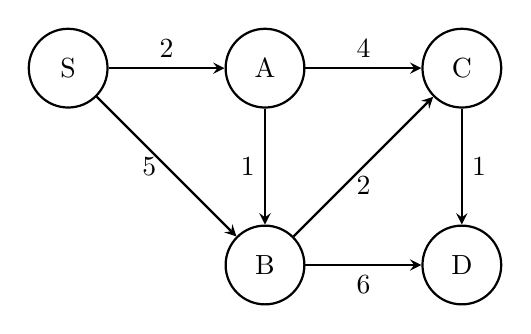
\begin{tikzpicture}[->, >=stealth, node distance=2.5cm, thick]
        % Nodes
        \node (S) [circle, draw, minimum size=1cm] {S};
        \node (A) [circle, draw, minimum size=1cm, right of=S] {A};
        \node (B) [circle, draw, minimum size=1cm, below of=A] {B};
        \node (C) [circle, draw, minimum size=1cm, right of=A] {C};
        \node (D) [circle, draw, minimum size=1cm, below of=C] {D};
    
        % Edges with weights
        \draw (S) -- (A) node[midway, above] {2};
        \draw (S) -- (B) node[midway, left] {5};
        \draw (A) -- (B) node[midway, left] {1};
        \draw (A) -- (C) node[midway, above] {4};
        \draw (B) -- (C) node[midway, below] {2};
        \draw (B) -- (D) node[midway, below] {6};
        \draw (C) -- (D) node[midway, right] {1};
    \end{tikzpicture}
\end{center}

Run Dijkstra�s algorithm starting from vertex \(S\) and list the order in which vertices are settled along with their final distances. Show detailed step-by-step iterations.

\vfill

\exercise
Provide an example of a graph where Dijkstra�s algorithm fails to produce correct shortest paths.
\babc
\item 
Describe a graph (with vertex names and edge weights) that includes a negative edge weight.
\item 
Explain why Dijkstra�s algorithm fails on this graph.
\eabc
\newpage

\exercise
Prove that if a graph contains no negative-weight cycles reachable from the source, the Bellman�Ford algorithm correctly computes the shortest-path distances after $|V|-1$ iterations of edge relaxations.
\vskip 0.1in\noindent
\textbf{HINT:} 
Your proof should follow the below outline.

\begin{itemize}
\item 
Prove that in a graph with no negative-weight cycles, any shortest path from the source to any vertex contains at most $|V|-1$ edges.
    
\item 
Prove that after the $i$-th iteration of edge relaxations, the algorithm correctly finds all shortest paths containing at most $i$ edges.
    
\item 
Prove that after $|V|-1$ iterations, all shortest paths must have been found, since any valid shortest path consists of at most $|V|-1$ edges.
    
\item 
Suppose a shorter path still exists after $|V|-1$ iterations. Prove that this would require a path with at least $|V|$ edges, implying a cycle. Conclude why this contradicts the assumption that there are no negative-weight cycles.
\end{itemize}

\vfill

\challenge 
\textbf{Shortest Paths with Edge Reversals.}
You are given a directed graph $G=(V,E)$ with positive edge weights, and two vertices $s,t \in V$.  
You are allowed to reverse the direction of \emph{at most one edge} in the graph. Your task is to compute the minimum possible distance from $s$ to $t$ after reversing zero or one edge.
\begin{enumerate}[(a)]
\item 
Describe an efficient algorithm to compute the shortest $s \to t$ distance if you are allowed to reverse at most one edge. Explain how you handle the possibility of reversing an edge optimally. 
\vskip 0.1in\noindent
\textbf{HINT:} 
Consider computing shortest paths from $s$ and to $t$ separately.
\item 
Suppose you reverse exactly one edge $(u,v)$. Express the new $s \to t$ distance in terms of:
\begin{itemize}
\item $d_s[u]$, the original shortest distance from $s$ to $u$,
\item $w(u,v)$, the weight of edge $(u,v)$, and
\item $d_t[v]$, the original shortest distance from $v$ to $t$ \emph{in the reversed graph}.
\end{itemize}
Explain why checking all edges using this formula finds the optimal edge to reverse.
    
\item
Write pseudocode for your algorithm, making it clear how many times you need to run Dijkstra�s algorithm (or an equivalent SSSP procedure) and on which graphs.
    
\item 
Analyze the runtime of your algorithm in terms of $|V|$ and $|E|$. Explain why your approach is asymptotically faster than naively trying all possible edge reversals and recomputing SSSP from scratch.
\end{enumerate}
\vfill
\end{document}